\section{Implementação em Produção} \label{implementacao_producao}
\subsection{Aplicação Desenvolvida}

A aplicação desenvolvida para produção foi construída em \textit{Python}, com uma interface gráfica implementada através da biblioteca \textit{Tkinter}.

Com o intuito de facilitar o processo de desenvolvimento do modelo final, decidiu-se que a aplicação não incluiria um modelo previamente definido e carregado automaticamente. Assim, para que a aplicação funcione corretamente, o utilizador deve selecionar manualmente o modelo pretendido, através de um botão localizado na barra de ferramentas da interface.

\begin{figure}[ht]
    \centering
    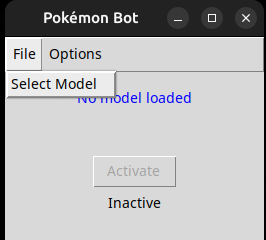
\includegraphics[width=0.3\linewidth]{imagens/carregamento_modelo.png}
    \caption{Interface principal da aplicação com o botão de carregamento do modelo}
    \label{fig:carregamento_modelo}
\end{figure}

De forma a tornar a aplicação mais flexível e reutilizável em outros contextos, foi ainda incluído um ecrã de configuração onde o utilizador pode personalizar algumas variáveis de funcionamento. As variáveis disponíveis para configuração são:

\begin{itemize}
    \item Intervalo de tempo entre capturas de ecrã (em milissegundos);
    \item Opção de guardar ou não as imagens capturadas;
    \item Opção de mostrar ou não na interface as imagens capturadas;
    \item Diretório onde as imagens capturadas serão armazenadas.
\end{itemize}

\begin{figure}[ht]
    \centering
    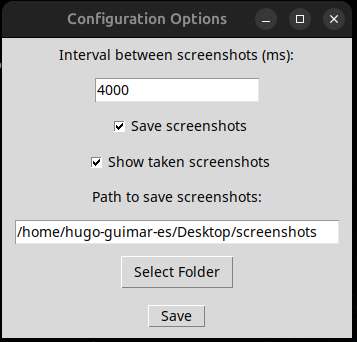
\includegraphics[width=0.4\linewidth]{imagens/configuracoes.png}
    \caption{Ecrã de configuração das variáveis da aplicação}
    \label{fig:configuracoes}
\end{figure}

Após o carregamento de um modelo, o botão de ativação da aplicação fica disponível. Quando ativada, a aplicação começa a capturar imagens do ecrã com a periodicidade definida, processa essas imagens através do modelo selecionado, e com base nos dados obtidos, move automaticamente o cursor do rato para interagir com a interface do jogo, selecionando as opções consideradas mais adequadas.

\begin{figure}[ht]
    \centering
    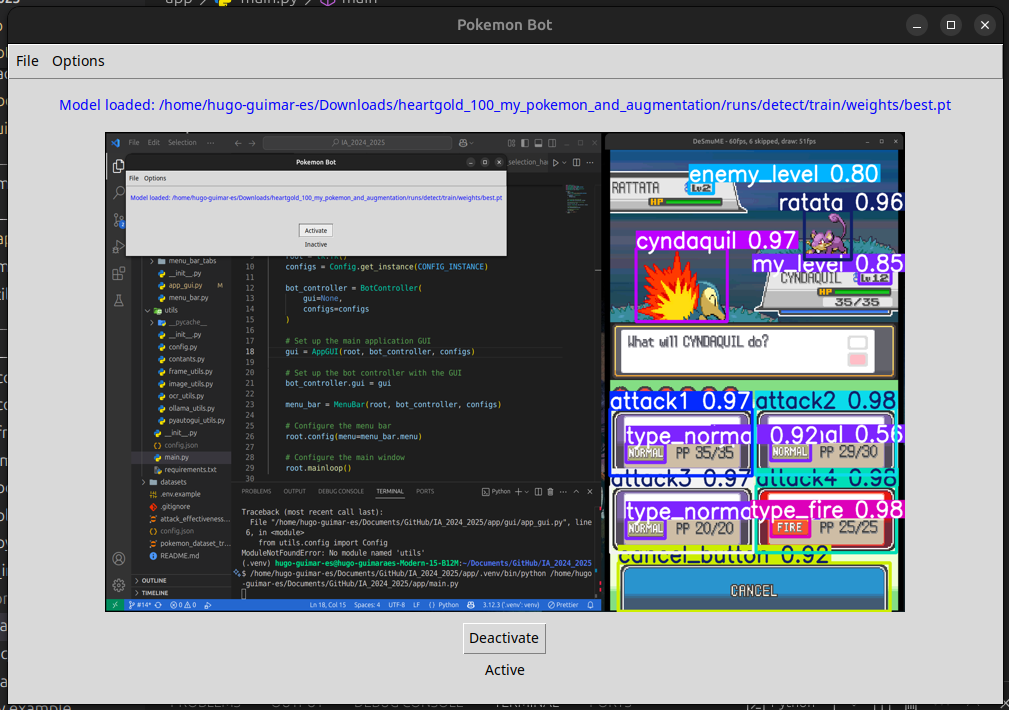
\includegraphics[width=1.0\linewidth]{imagens/aplicacao_em_execucao.png}
    \caption{Aplicação em execução após o carregamento do modelo}
    \label{fig:aplicacao_em_execucao}
\end{figure}

\subsection{Limitações da Aplicação}
Como foi utilizado um modelo de linguagem (LLM) e um reconhecimento ótico de caracteres (OCR) em produção, o bot acaba por demorar bastante tempo a executar as ações. Além disso, mesmo otimizando as instruções do modelo de linguagem, este continua a gerar respostas muito longas, o que, em alguns casos, obriga a executar o modelo novamente, uma vez que não foi possível interpretar a resposta anterior, atrasando ainda mais a tomada de decisão do bot.

Para realizar a movimentação automática do cursor, foi utilizada a biblioteca \textit{PyAutoGUI}. No entanto, esta funcionalidade pode apresentar limitações em determinados sistemas operativos.

No sistema operativo \textit{Windows}, poderá ser necessário executar o script com permissões de administrador, caso contrário, poderão ocorrer restrições na interação com o sistema.

Em sistemas \textit{Linux}, a aplicação poderá não funcionar corretamente se estiver a ser utilizado o servidor gráfico \textit{Wayland}, uma vez que este impõe fortes restrições quanto à interação entre aplicações. Para garantir o funcionamento da aplicação, recomenda-se a utilização do servidor gráfico \textit{Xorg} ou de uma outra alternativa que não seja tão restritiva.

